\documentclass[a4paper, norsk, twoside, 10pt]{article}

\usepackage{epsfig}
\usepackage{graphicx}
\usepackage{gensymb}
\usepackage{amsmath}
\usepackage{amsthm}
\usepackage{amssymb}
\usepackage[utf8]{inputenc}
\usepackage[a4]{}
\usepackage{float}
\usepackage{listings}
\usepackage{pgfplots}
\usepackage{pgffor}

\date{\today} 
\title{Lab 6 \\ eksamen 2014}
\author{Elsie Mestl}

\begin{document}
\maketitle
\section*{Oppgave 1:}
\subsection*{a)}
Har at R3 og R2 står i parralell og at denne samlede motstanden står i serie med R1. Gir at:
\begin{align*}
  R_{total} &= R_{1} + \frac{1}{\frac{1}{R_{2}} + \frac{1}{R_{3}}}\\
  &= 5 \cdot 10^{3} \Omega + \frac{1}{\frac{1}{15 \cdot 10^{3}  \Omega} + \frac{1}{10 \cdot 10^{3}  \Omega}}\\
  &= 5 \cdot 10^{3} \Omega +\frac{1}{\frac{1}{6000 \Omega}} \\
  & = 5 \cdot 10^{3} \Omega + 6 \cdot 10^{3} \Omega = 11k \Omega
\end{align*}
R1, R2 og R3 kan altså byttes ut med en $11k\Omega$ motstand


\subsection*{b)}
Ser at spenningen $V_{in}$ er en AC spenning gitt ved $V_{in} = 1+ 2\sin{t}$. Det tilsvarer altså en AC spenning med DC-offset = 1V og en peak-peak amplitude på 4V.

Dette gjør at $I_{tot-DCoffset}$ vil har en DC offset på
\[I_{DC-offset} = \frac{V_{in-DCoffset}}{R_{total}} = \frac{1}{11 \cdot 10^{3}}A\]
Og en peak-to-peak verdi på
\[I_{pp} = \frac{V_{in-pp}}{R_{total}} = \frac{4}{11 \cdot 10^{3}}A\]

Har at siden $I_{R1}$ er seriekoblet til hele kretsen er $I_{R1} =I_{tot}$ som git en $I_{R1}$ på:

\[I_{R1} = \frac{1}{11 \cdot 10^{3}}\ + \frac{4}{22 \cdot 10^{3}} \sin{t} = \frac{1}{11\cdot 10^3}(1 + 2\sin{t})A\]


\subsection*{c)}
Maks offsetet til $V_{out}$ er når $V_{in}$ er på maks peak, vil si $V_{in-maks} = 1 +2 = 3$ og tilsvarende for min peak $V_{in-min} = 1 -2 = -1$
$V_{out}$ er $V_{in}$ minus spenningsfallet over begge motstandene koblet i paralell. Dette tilsvarer

\[R_{parallell} = \frac{1}{\frac{1}{R_{2}} + \frac{1}{R_{3}}}\]
\[V_{out} = V_{in} - V_{R_{parallell}} = V_{R1} = I_{R1}\cdot R_{1} =  \frac{1}{11\cdot 10^3}(1 + 2\sin{t}) \cdot 5 \cdot 10^{3} \]
Gir:
\begin{align*}
  V_{out-maks} &=  \frac{5}{11}(3) = 1.36 V \\
  V_{out-min} &= \frac{5}{11}(-1) = -0.45 V
\end{align*}


\subsection*{d)}
Antar skrivefeil, der det står at A skal skrives som en funksjon av $R_{1}, R_{2}$ og $X_{C}$ antar de mener R3 og ikke R1\\
La:
\[Z_{total} = \sqrt{X_{C}^{2} + R_{parallell}^{2}} \Omega\]
 
Har at: \[A = \frac{V_{out}}{V_{in}} = \frac{V_{C}}{1+ 2\sin{t}} = \frac{I_{C} \cdot X_{C}}{I_{tot} \cdot Z_{total}}
= \frac{I_{total} \cdot X_{C}}{I_{tot} \cdot Z_{total}}= \frac{X_{C}}{Z_{totalt}}\]


\subsection*{e)}
Har at: \[X_{C} = \frac{1}{2\pi f \mathrm{C}} = \frac{1}{100\pi f 10^{-6}} \Omega\]
Ser at når $\lim_{f \to \infty}$ så er $X_{C} \approx 0$ altså vil $Z_{total}$ gå mot $R_{prarallell}$ Men telleren i A vil gå mot 0, og dermed har vi at A vil gå mot 0. Når $\lim_{f \to 0}$ blir  $X_{C} \approx \infty$ som gjør at $R_{parallell}$ ikke spiller noe rolle, for altså $\frac{X_{C}}{X_{C}}$ som gir 1.\\*
Har altså at:
\[A \in <0,1>\]


\newpage
\section*{Oppgave 2}
\subsection*{a)}

Finner R ved å lese av strøm-verdien ved de gitte spenningene og deretter bruker Ohms-lov:

\begin{align*}R &= \frac{V}{I}\\
  \\
  R &= \frac{-60 V}{5nA} = 12 G \Omega\\
  R &= \frac{0.5}{0.8mA} = 625 \Omega \\
  R &= \frac{0.8}{6.5mA} = 123.1 \Omega \\
\end{align*}



\subsection*{b)}
Ser at dette er samme kretsen som i Oppgave1 men hvor $R_{parallell}$ er byttet ut med en diode og $R_{1}$ har økt til $10k \Omega$ \\
Har altså samme bregninger som i oppgaven over:
\begin{align*}
  V_{toal-maks} &= 3\\
  V_{toal-min} &= -1\\
  \\
  I_{R} &= I_{total} = \frac{V_{total}}{R_{total}}
\end{align*}
Siden $R_{total}$ er summen av motstanden R og motstanden til dioden som varierer med spenningen over den. Siden vi kan regne dioden som en ideel diode kan vi si at strømmen gjennom den er 0 frem til V= 0.7V Dette gjør at:
\[I_{total-min} = 0 \]
Når $V \geq 0.7$ så er grafen lineær. Altså er I lineært avhengig av V over dioden. Når $V_{total} = 3V$ så er strømmen gjennom R gitt ved $V_{total-maks}$:
\[V_{R} = V_{total} - 0.7 = 3-0.7 = 2.3V\]
Gir
\[I_{total-maks} =  \frac{V_{total-maks}}{R_{total}} = \frac{2.3}{10k} = 2.3mA\]





\subsection*{c)}

Kretsen er en NAND-implementasjon. Det ser vi ved at hvis både $V_A$ og $V_B$ er høye (altså 5V hver seg) så vil diodene være stengt og all spenningen pluss det litt dioden utgir siden de er reversebiased gå til basen på transistoren. Dette vil føre til at den er åpen, altså leder strøm, og dermed ser vi at all spenningsfallet må skje over $R_2$ og $V_{out}$ vil altså være på 0V som tilsvarer logisk lav (0).\\
Ellers hvis $V_A$ eller $V_B$ er lave vil all strømmen bli trukket ut via denne dioden, for nå vil den kunne lede. Dermed vil spenningen ved basen være for lav til at transistoren vil åpne seg, altså vil all spenningen fra $V_{CC}$ måtte gå ut via $V_{out}$ som impliserer 5V som tilsvarer logisk høy (1). \\
Alså vi får følgende sannhetsverditabell, tabellen for en NAND port:

\begin{tabular}{|l|c||r}
  \hline
  V_A & V_B & V_{out} \\
  \hline
  0 & 0 & 1 \\
  0 & 1 & 1 \\
  1 & 0 & 1 \\
  1 & 1 & 0 \\
  \hline
\end{tabular}
  



\newpage

\section*{Oppgave 3}
\subsection*{a)}
\subsubsection*{1.}
Kretsen er en forsterker med negativ tilbakekobling. Det er en sumerende forsterker; som gir ut og forsterker summen av innspenningene. 



\subsubsection*{2.}
Har at:
\[V_{out} = \frac{-R_{f}}{R_{prallell}} (V_{1} + V_{2} + V_{3})\]
Hvis kretsen ikke hadde vært en forsterker ville $V_{out} = V_{1} + V_{2} + V_{3}$. Forstrekningen beholder frekvens altså det eneste som endres er amplituden. Altså må den forsterkete faktoren være:


\begin{align*}
  A &= \frac{-R_{f}}{R_{prallell}} \\
  &= \frac{-14.1k\Omega}{\frac{4.7k\Omega}{3}}  = \frac{-3*14.1}{4.7}  = -9
\end{align*}

Det negative fortegnet forteller at forsterkning er 180\degree faseforskøvet



\subsubsection*{3.}
\begin{align*}
  V_{1} &= 1V \\
  V_{2} &= -2V\\
  \\
  V_{out} &= -8V
\end{align*}
Siden:
\[V_{out} = \frac{-R_{f}}{R_{prallell}} (V_{1} + V_{2} + V_{3})\]
Og vi har at forsterkningen er -9 har vi:
\begin{align*}
  V_{3} &= \frac{V_{out}}{-9}- V_{1} - V_{2} \\
  &= \frac{-8}{-9}- 1 + 2 = 1.89 V
\end{align*}


\subsection*{b)}
\subsubsection*{1.}
Et passivt filter består kun av passive deler (R, C, L) mens et aktivt filter består av et passivtfilter og en forsterker. \\
Hovedforskjellen mellom aktive og passivefiltere er at et passivt filter har maks en forstrekning på A=1 i tillegg har passive filtere en mye slakere rolloff. Dette kommer av at en forsterker kun forsterker et signalt, og det lineært, dvs forskjellen mellom topp og bånn er mye større i et aktivt filter enn et passivt ett men tiden det tar å komme fra A til B er lik, derfor har vi at rolloffen til aktive filtere er brattere.

\subsubsection*{2.}
Kretsen er et lavpass filter, dvs det er hovedsaklig spenningen ved lave frekvenser som slipper gjennom. Så ved å sende inn et DC-signal eller et signal med lav frekvens. \\
Siden vi har at første delen er et lavpassfilter så vil de signalene vi sender gjennom bare gå rett gjennom. Forsterkeren har en forstrekningsgrad på 1 for lave frekvenser (siden lavpassfilter) og ingen faseforsyvning siden signalet er koblet til den possitive inngangen til opampen. Kretsen er derfor en spenningsfølger også kalt en buffer. Det den gjør er at man kan sette på en ekstra load på $V_{out}$ uten at det vil endre på $V_{in}$.



\subsubsection*{3.}
Hovedsakelig svart på i oppgaven over, men i passområdet er A = 1. \\
Grunnen til at den ikke er større er fordi det ikke er koblet til noen komponenter i tilbakekoblingen, derfor vil spenningen som blir sendt tilbake være lik den spenningen som blir sendt inn. Altså vil det ikke være noen forsterkning av inngangssignalet, altså A = 1.




\subsection*{c)}
Siden kretsen er en integrator vet vi at utsagnssignalet er intergralet av inngangssignalet. For en ideel krets får vi følgende resultat:\\
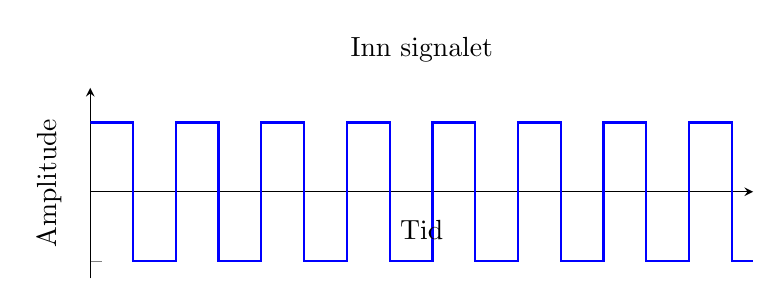
\begin{tikzpicture}
  \begin{axis}[
      width=10cm ,
      height=4cm,
      x axis line style={-stealth},
      y axis line style={-stealth},
      title={Inn signalet},
      xticklabels={},
      yticklabels = {},
      ymax = 1.5,xmax=15.5, xmin = 0,
      axis lines*=center,
      xlabel={Tid},
      ylabel={Amplitude},
      ylabel near ticks
    ]
    \addplot+[thick,mark=none,const plot]
    coordinates
    {(0,1) (1,-1) (2,1) (3,-1) (4,1) (5,-1) (6,1) (7,-1) (8,1) (9,-1) (10,1) (11,-1) (12,1) (13,-1) (14,1) (15,-1) (15.5, -1)};
    enlarge x limits=true
  \end{axis}z
\end{tikzpicture}

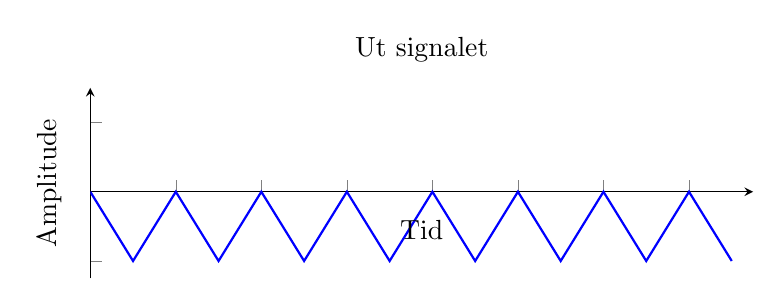
\begin{tikzpicture}
  \begin{axis}[
      width=10cm ,
      height=4cm,
      x axis line style={-stealth},
      y axis line style={-stealth},
      title={Ut signalet},
      xticklabels={},
      yticklabels = {},
      ymax = 1.5,xmax=15.5, xmin = 0,
      axis lines*=center,
      xlabel={Tid},
      ylabel={Amplitude},
      ylabel near ticks
    ]
    \addplot+[thick,mark=none]
    coordinates
    {
     (0,0) (1,-1) (2,0) (3,-1) (4,0) (5,-1) (6,0) (7,-1) (8,0) (9,-1) (10,0) (11,-1) (12,0) (13,-1) (14,0) (15,-1)};
    enlarge x limits=true
  \end{axis}z
\end{tikzpicture}



\subsection*{d)}
Antar det menes at ingangssignalet fremdeles ansees som ideelt altså er det kun opampen som er ikke ideel, og vi er gitt følgende forutsetninger: \[V_{out} > 0, \quad V_{in} = 0\]
Det betyr at utgangssignalet er større enn ing


FINN UT AV DENNE!



\section*{Oppgave 4}
\subsection*{a)}
Målte verdier
\begin{align*}
V_{B} &= 3V\\
V_{C} &= 9V\\
\\
V_{TH} &= 0.7V
\end{align*}

Finn feilen.\\
Siden $V_{CC} = V_{C}$ har vi at det ikke går noe strøm i transistoren (men det var også til å forstå av oppgaveteksten). Har også at siden emitoren er koblet til jord så er $V_{E} =0$. Dette gjør at $V_{BE} > V_{TH}$ og transistoren burde derfor lede strøm. Det tyder derfor på at feilen ligger i basen.


\subsection*{b)}
Poenget med $R_{C}$ er at spenningen inn til kolektoren blir mindre, og etterhvert som tranistoren leder mer og mer strøm så vil spenningstilføreslen til $V_{C}$ øke, som igjen fører til at den leder mer strøm.
\\
Ved å ha en motstand etter emitteren hever man også spenningen til emitteren til alltid å måtte være på samme nivå som jord. M.a.o. ved å koble inn de to mitstandene kan man sende inn et større signal enn mann ellers kunne uten å ødelegge kretsen.
\\
Kretsen er en `Voltage-divider bias'




\subsection*{c)}
\begin{align*}
  I_{E} &= 4mA\\
  I_{B} &= 10\mu A
\end{align*}

Finn $I_{C}$ og $\beta$:\\
\begin{align*}
  &I_{C} = \beta \cdot I_{B} \\
  &I_{E} = I_{C} + I_{B} \\
  \\
  &I_{C} = I_{E} - I_{B} = 4\cdot 10^{-3} - 10\cdot 10^{-6} = 3.99mA \\
  &\beta = \frac{I_{C}}{I_{B}} = 399
\end{align*}


\subsection*{d)}
Ved å minske $R_{2}$ vil det meste av spenningsfallet skje over $R_{1}$ og dermed vil $V_{B}$ minke. \\
Har at: \[V_{TH} = 0.7V \]
Den minste verdien for $R_{2}$ må altså være slik at $V_{BE} \geq 0.7$ og siden emitteren ikke er koblet direkte til ground så må altså:
\[V_{B} = V_{BE} +V_{E} = 0.7 + V_{E}\]
Og siden transistoren ikke leder noe strøm før $V_{BE} > 0.7$ og dermed er $V_E = 0V$ før dette skjer. Altså må $V_B = 0.7$. Da har vi en vanlig spenningsdeler og vi har følgende formel.
\begin{align*}
  V_{CC} &= R_{total}I \\
  I &= \frac{25}{44k\Omega + R_2}\\
  \\
  V_{R2} &= 0.7V = R_2I = \frac{25R_2}{44k\Omega + R_2} \\
  0.7(44k\Omega + R_2) &= 25R_2 \\
  25R_2 -0.7R_2 &= 24.3R_2 = 30.8k\Omega \\
  R_2 &= 1.3k\Omega
\end{align*}


\subsection*{e)}

I den første kretsen er faseforskyvningene mellom $V_{in}$ og $V_{out}$ $180\degree$ dette er fordi når $V_{in}$ øker så vil transistoren lede mer strøm, det vil si motstanden over transistoren minker. Og etter oms-lov vil da spenningen over $V_E$ øke og da må den minke over $V_C$. Dette gjelder også andre veien.
\\
Den samme logikken gjelder for den andre kretsen, men har er outputen på $V_E$ og derfor vil ingang og utgangssignalet ligge i samme fase. 



\section*{Oppgave 5}
\subsection*{a)}
4. Det er det som er poenget med en `algebraisk sum', retningen har ingenting å si.
\subsection*{b)}
5. Det inverse til reaktans er impendans og reaktiv er inverse til kapasativ. SJEKK DENNE!
\subsection*{c)}

\subsection*{d)}

\subsection*{e)}

\end{document}
